\mychapter{Teori}

\section{Kryptering}
Kryptering handlar om att gömma information för att förhindra att andra än den menade mottagaren kan läsa informationen.
Detta genomförs i dagens samhälle genom olika typer av krypteringsalgoritmer. Dessa algoritmer kan ses som både komplicerade
och för virrande men bygger på enkla principer. En krypteringsalgoritm tar in en text och en nyckel och ger sedan tillbaka en
skiffertext, vilket då är en krypterad version av den ursprungliga texten.\footfullcite{kryptering}

För att den menade mottagaren ska kunna läsa skiffertexten sedan så behöver hen ha en nyckel samt köra samma krypteringsalgoritm
i dekrypterings läge. Bland de vanligaste typerna av krypteringsalgoritmer finns \nameref{sec:symmetric-asymmetric-encryption},
vilket bland annat innefattar algoritmer som \acrshort{aes} och \gls{rsa}.\footcite{kryptering}

\section{Blockskiffer}
\label{sec:blockskiffer}
Blockskiffer är en krypteringsalgoritm som verkar på block av data med en fast storlek.
blockskiffer används bland annat som en av grundkomponenterna i kryptografiska protokoll som \acrfull{tls} och \acrfull{ssl}
som används för att kryptera data som skickas över internet bland annat.\footfullcite{blockskiffer-ref}

En ut av de största problemen med Blockskiffer är dock att oavsett hur säkra dom är så passar det bara att använda
för kryptering av enskilda block med en nyckel, vilket skiljer sig från något som ett \gls{streamcipher}.
På grund av detta har en mängd olika körlägen utvecklats för att på så sätt göra de möjlig att utnyttja
blockskiffer för att kryptera större mängder data med en nyckel.\footcite{blockskiffer-ref}

Blockskiffer används däremot inte bara för kryptering utan kan även användas i olika typer av \gls{hashfunktion}er  % needs glossary entry
och \gls{pseudoslump} nummer generatorer bland annat då blockskifferets resulterande skiffertext ser ut att vara slumpmässig.\footcite{blockskiffer-ref}
% need to add more

\subsection{Körlägen}
Körlägen inom kryptografin kan man se som algoritmer som appliceras i användningen av
blockskiffer eftersom dessa endast är användbara för säker kryptering av ett litet block med bestämd längd.
Körlägena gör de då möjligt att istället kunna använda blockskiffer på större data mängder.
Detta löser körlägen på olika sätt beroende på hur man vill använda blockskiffer algoritmen samt hur
mycket man ör villig att kompromissa med säkerheten i förhållande till hastighet.\footfullcite{modesofoperation}

Ett ut av sätten som körlägen löser problemet med att applicera blockskiffer algoritmer på
större data mängder är att dom använder sig av en så kallad \acrfull{iv}. Det är en unik sekvens
av bytes som används för att säkerställa att samma data mängd aldrig kommer att generera samma
krypterade skiffertext.\footcite{modesofoperation}

\acrshort{iv} kan användas på många sätt från att introduceras genom en
\gls{xor}-operation med första blocket och sedan kedja ihop och göra samma sak med nästkommande
block fast med resultatet från den första operationen precis som i \acrshort{cbc}. Detta gör att blocken blir beroende av varandra
plus att samma information som krypteras flera inte kommer ge samma resultat även fast man använder samma
nyckel.\footcite{modesofoperation}

\subsubsection{ECB}
\acrfull{ecb} är en av det enklaste blockchiffer körlägena som finns.
\acrshort{ecb} i sig är ganska lätt att förstå och bygger i huvudsak bara på
att man delar upp den data man vill kryptera i delar kallade block och tar sedan varje
block för sig och kör genom algoritmen, vilket tydligt visas i
figur \ref{fig:ecb-mode-enc} \& \ref{fig:ecb-mode-dec}.
\footcite{modesofoperation}

Figur \ref{fig:ecb-mode-enc} visar hur \acrshort{ecb} fungerar vid kryptering.
Här visas hur varje block för sig krypteras med hjälp av en blockchiffer algoritm
tillsammans med den givna nyckeln.

\begin{figure}[H]
    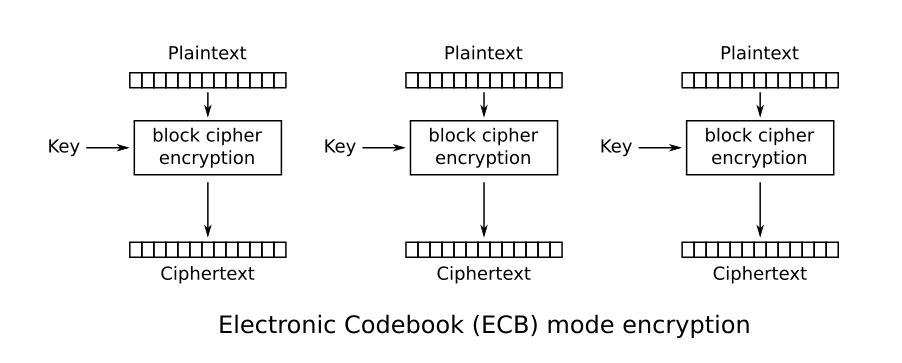
\includegraphics[width=\textwidth]{ECB_encryption.png}
    \caption{\acrlong{ecb} kryptering \cite{ecb-mode-enc-ref}}
    \label{fig:ecb-mode-enc}
\end{figure}

Figur \ref{fig:ecb-mode-dec} visar istället hur \acrshort{ecb} fungerar vid
dekryptering, vilken är en till stort sett identisk operation med det enda undantaget
att blockchiffret körs i dekrypterings läge istället för krypterings läge. % May need reformulating!!

\begin{figure}[H]
    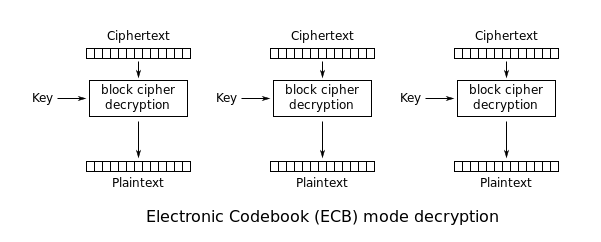
\includegraphics[width=\textwidth]{ECB_decryption.png}
    \caption{\acrlong{ecb} dekryptering \cite{ecb-mode-dec-ref}}
    \label{fig:ecb-mode-dec}
\end{figure}

På grund av \acrshort{ecb} körlägets simplicitet så finns det dock även ett ganska
stort problem med detta körläge. Det handlar om att \acrshort{ecb} inte på något
sätt förhindrar att två block med samma innehåll som krypteras inte resulterar i
ett identiskt krypterat block.\footcite{modesofoperation}

Vad detta innebär är att för större mängder data
är att det börjar bildas mönster i skiffertexten. Detta är något som väldigt
tydligt visar sig ifall man krypterar en bild, vilket går att se när man jämför
figur \ref{fig:pi-original} \& \ref{fig:pi-ecb}.
Det här faktumet är även varför \acrshort{ecb} inte är ett säkert körläge
och därför inte används näst intill aldrig i praktiken.\footcite{modesofoperation}

\acrshort{ecb} har däremot även sina fördelar då de bland annat kan parallelliseras
både när de gäller krypteringen och dekrypteringen. Detta samt att \acrshort{ecb}
även gör de möjligt att slumpmässigt dekryptera enskilda block av en skiffertext
utan att man behöver dekryptera hela texten.\footcite{modesofoperation}

\subsubsection{CBC}
\acrlong{cbc} är ett av de mest vanligen använda körlägena för många blockchiffer.
Till skillnad från \acrshort{ecb} så förhindrar \acrshort{cbc} att två block med
samma innehåll kan ge samma krypterade block. Detta gör \acrshort{cbc} genom att
lägga till ett extra steg utöver vad som finns i \acrshort{ecb}. Steget
är en \gls{xor}-operation mellan det krypterade blocket nästkommande block innan
de körs genom blockchiffer algoritmen.\footcite{modesofoperation}
Matematisk sett kan detta formuleras såhär:

\begin{equation}
    \label{eq:cbc-encryption}
    \begin{aligned}
        &S_i = K_n(B_i \oplus S_{i-1})\\\nonumber
        &S_0 = IV
    \end{aligned}
\end{equation}

Där $S_i$ är det krypterade blocket(skiffertexten), $B_i$ är det blocket som ska krypteras,
$K_n$ är blockchiffer algoritmen där $n$ står för nyckeln och $S_{i-1}$ är
det krypterade blocket före det blocket som ska krypteras. \acrshort{iv} är en
\acrfull{iv} som används vid krypteringen av de första blocket då de inte finns
något föregående block att använda. $i$ står för index där de första blocket har
index värdet 1. Hela den här processen kan även ses i figur \ref{fig:cbc-mode-enc}.

\begin{figure}[H]
    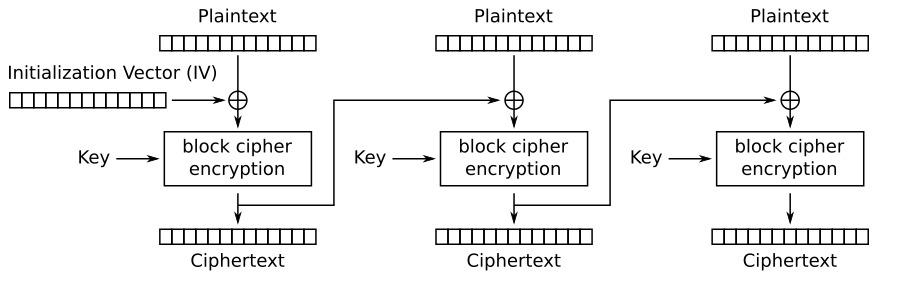
\includegraphics[width=\textwidth]{CBC_encryption.png}
    \caption{\acrlong{cbc} kryptering \cite{cbc-mode-enc-ref}}
    \label{fig:cbc-mode-enc}
\end{figure}

När de gäller dekrypterings processen för \acrshort{cbc} så bär den precis som för
\acrshort{ecb} stora likheter med krypterings processen. Det två skillnaderna som
finns är att blockchiffert körs i dekrypterings läge istället för krypterings läge.
Samt att för varje block så genomförs en \gls{xor}-operation mellan det dekrypterade
blocket och föregående block innan dekrypteringen av blocket.\footcite{modesofoperation}
Även detta går att både matematiskt formulera och visuellt visa såhär:

\begin{equation}
    \label{eq:cbc-decryption}
    \begin{aligned}
        &B_i = K_n(S_i) \oplus S_{i-1}\\\nonumber
        &S_0 = IV
    \end{aligned}
\end{equation}

\begin{figure}[H]
    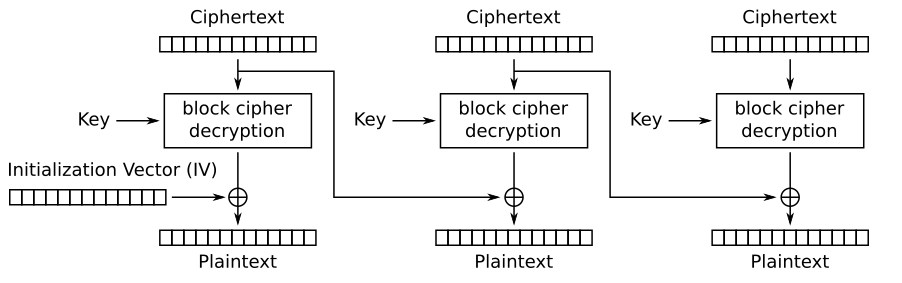
\includegraphics[width=\textwidth]{CBC_decryption.png}
    \caption{\acrlong{cbc} dekryptering \cite{cbc-mode-dec-ref}}
    \label{fig:cbc-mode-dec}
\end{figure}

Fördelarna som kommer från den extra operationen i \acrshort{cbc} till skillnad
från \acrshort{ecb} är då att varje block blir beroende av föregående block.
Detta innebär att dom mönster som kunde dyka upp i \acrshort{ecb} inte längre
kan uppstå, vilket då gör \acrshort{cbc} till ett mer säkert körläge än \acrshort{ecb}.
Dock kräver cbc en ytterligare faktor för att se till så att inte olika medelanden
kan ge samma krypterade block. Därav så krävs en \acrfull{iv} som används vid första
blocket.\footcite{modesofoperation}

\acrshort{cbc} är dock inte prefekt och har i sig också några nackdelar. Där ibland
exempelvis de faktum att en incorrect \acrshort{iv} leder till att de första blocket
inte kan dekrypteras korrekt, detta påverkar dock inte de resterande blocken. På grund
av det så kan man exempelvis lösa problemet genom att första blocket bara innehåller
någon typ av fyllnad, vilket då gör dekrypteringen möjlig utan tillgång till \acrshort{iv}.\footcite{modesofoperation}

Utöver detta så begränsas även \acrshort{cbc} till att bara vara parallelliserbar under
dekrypteringen och inte krypteringen, vilket är en konsekvens av att varje block i \acrshort{cbc}
är beroende av föregående block. \acrshort{cbc} behåller dock fortfarande möjligheten
som \acrshort{ecb} har att slumpmässigt dekryptera enskilda block utan att behöva
dekryptera hela skiffertexten.\footcite{modesofoperation}

\subsubsection{OFB}
\acrlong{ofb} är ett ytterligare körläge som skiljer sig en del från \acrshort{ecb}
och \acrshort{cbc} som  redan presenterats. Den största skillnaden från det andra
körlägena är att \acrshort{ofb} inte använder blockchiffer algoritmen för att kryptera
eller dekryptera blocken. Istället så körs \acrshort{iv} genom blockchiffer algoritmen
och den resulterande \gls{keystream} tillförs sedan genom en \gls{xor}-operation till
blocket som ska krypteras eller dekrypteras.\footcite{modesofoperation}

Tack vare \gls{xor}-operationens symmetriska natur så är så väl krypteringen som
dekrypteringen av \acrshort{ofb} identisk, vilket även visas i figur \ref{fig:ofb-mode-enc}
\& \ref{fig:ofb-mode-dec}:

\begin{figure}[H]
    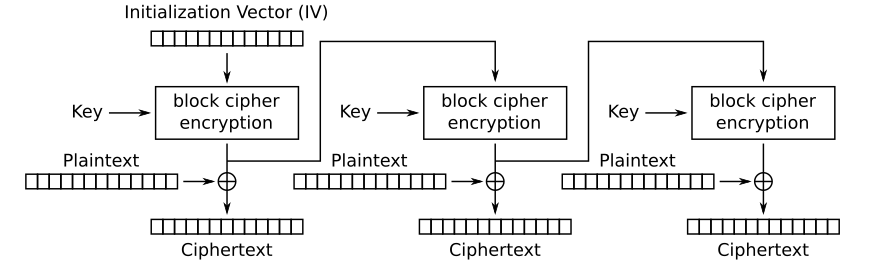
\includegraphics[width=\textwidth]{OFB_encryption.png}
    \caption{\acrlong{ofb} kryptering \cite{ofb-mode-enc-ref}}
    \label{fig:ofb-mode-enc}
\end{figure}

\begin{figure}[H]
    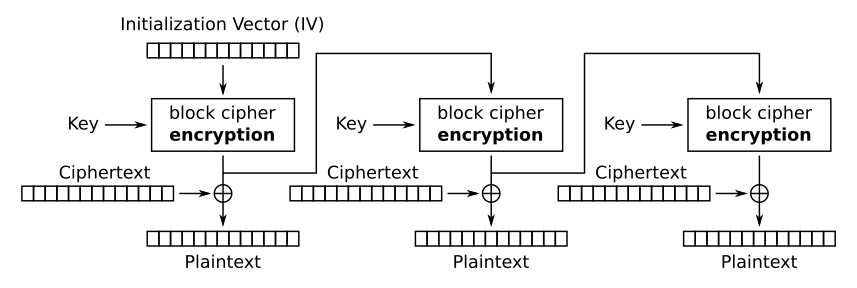
\includegraphics[width=\textwidth]{OFB_decryption.png}
    \caption{\acrlong{ofb} dekryptering \cite{ofb-mode-dec-ref}}
    \label{fig:ofb-mode-dec}
\end{figure}

Utöver detta kan man även matematiskt beskriva \acrshort{ofb}, vilket visas i ekvationen
nedan:

\begin{equation}
    \label{eq:ofb-encryption}
    \begin{aligned}
        &S_i = B_i \oplus O_i\\\nonumber
        &B_i = S_i \oplus O_i\\
        &O_i = K_n(I_i)\\
        &I_i = O_{i-1}\\
        &I_0 = IV
    \end{aligned}
\end{equation}

Här visas \acrshort{ofb} körläget matematiskt där $S_i$ är det krypterade blocket,
$B_i$ är blocket som ska krypteras och $I_0$ är \acrshort{iv}. Men här finns Även
$O_i$ som man kan säga är själva \gls{keystream} som används för att kryptera eller
dekryptera blocket. $O_i$ i sin tur bygger då på att $O_{i-1}$ körs genom blockchiffer
algoritmen igen och sedan används för nästa blocks kryptering.

På grund av att \acrshort{ofb} är utformat på det här sättet och att själva blocken som
ska krypteras inte används fram till sista steget så är det möjligt att genomföra blockskiffer
operationerna i förväg, vilket gör det möjligt att även parallellisera \acrshort{ofb}. Dock
kan \acrshort{ofb} inte parallelliseras ifall man inte gör blockskiffer operationerna
i förväg. Utöver detta saknar även \acrshort{ofb} möjligheten att slumpmässigt dekryptera
enskilda block utan att behöva dekryptera hela skiffertexten.\footcite{modesofoperation}

\section{Symetrisk \& Asymmetrisk Kryptering}
\label{sec:symmetric-asymmetric-encryption}
Symetrisk och asymetrisk kryptering handlar om hur nycklar används i olika
krypteringsalgoritmer. För symetriska krypterings algoritmer så betyder detta
att samma nyckel är vad som används för både kryptering och dekryptering. Medans
asymetrisk kryptering bygger på att man använder olika nycklar för kryptering och
dekrypterings processerna.\footfullcite{symencrypt}

De symetriska krypterings algoritmernas huvudsakliga nackdel ligger i de faktum att
de krävs en delad känd nyckel mellan båda parter. Detta är något som Asymetriska
krypterings algorithmer inte behöver, vilket har lett till att man ofta använder
asymetriska krypterings algoritmer för att sköta nyckelutbytet för de symetriska
krypterings algoritmerna. Anledningen till detta är att det symetriska krypterings
algoritmerna ofta är bättre för större data mängder då dom bland annat behöver mycket
kortare nyckellängder.\footcite{symencrypt}

Exempel på symetriska krypterings algoritmer är bland annat \acrshort{aes} och
\acrshort{des} var av \acrshort{aes} kommer förklaras djupare senare i denna rapport.\footcite{symencrypt}
Medans exempel på asymetriska krypterings algoritmer är bland annat \gls{rsa}.\footfullcite{rsa-ref}

\section{AES}

Som nämnts tidigare i \nameref{sec:aes-uppkomst} bygger \acrshort{aes} standarden på en variant av Rijndael \nameref{sec:blockskiffer} algoritmen
skapad av Vincent Rijmen och Joan Daemen. \acrshort{aes} är en symetrisk \nameref{sec:blockskiffer} krypterings algoritm som utformades för att ersätta
\acrshort{des} som då var den dominerande krypterings algoritmen. \acrshort{aes} är en av de mest använda krypterings algoritmerna idag
och används bland annat i säkerhetsprotokoll så som \acrfull{wpa2}\footfullcite{wpa2_ref}. \acrshort{aes} går att dela upp i tre olika varianter
som alla är baserade på samma grundläggande struktur. Dessa varianter är \nameref{sec:aes-128bit}, \nameref{sec:aes-192bit} och \nameref{sec:aes-256bit} som huvudsakligen
skiljer sig från varandra när det kommer till längden av krypteringsnyckeln samt antalet rundor som genomförs i algoritmens krypterings process.\footfullcite{aes_wiki}

Även själva algoritmen kan delas upp i ett antal olika delar som alla har olika syften. Dessa delar är \nameref{sec:aes-addroundkey}, \nameref{sec:aes-subbytes}, \nameref{sec:aes-shiftrows},
\nameref{sec:aes-mixcolumns} och \nameref{sec:aes-key-expansion} som alla kommer att förklaras mer detaljerat i de följande sektioner. \nameref{sec:aes-key-expansion} delen kan även
delas upp ytterligare i tre olika varianter som är \nameref{sec:aes-key-expansion-128bit}, \nameref{sec:aes-key-expansion-192bit} och \nameref{sec:aes-key-expansion-256bit} beroende
på vilken av de tre \acrshort{aes} varianterna som används.\footcite{aes_wiki}

Utöver detta så bygger \nameref{sec:aes-key-expansion} på tre operationer vilka är \nameref{sec:aes-subword}, \nameref{sec:aes-rotword} och
\nameref{sec:aes-rcon} som också kommer att förklaras mer detaljerat i de följande sektioner.\footcite{aes_wiki} För att förstå vissa av dessa delar
så kommer det däremot krävas en förklaring av både \nameref{sec:aes-sbox} och \nameref{sec:finite-fields} som kommer att förklaras först.

\subsection{Finite Fields}
\label{sec:finite-fields}

\subsubsection{AES Finite Field $GF(2^8)$}
\label{sec:aes-finite-field}


\subsection{AES S-Box}
\label{sec:aes-sbox}


\subsection{Struktur}
\label{sec:aes-structure}


\subsubsection{SubBytes operation}
\label{sec:aes-subbytes}
SubBytes operationen bygger på ...

\subsubsection{ShiftRows operation}
\label{sec:aes-shiftrows}


\subsubsection{MixColumns operation}
\label{sec:aes-mixcolumns}


\subsubsection{AddRoundKey operation}
\label{sec:aes-addroundkey}


\subsection{Nyckel utökning}
\label{sec:aes-key-expansion}


\subsubsection{RotWord}
\label{sec:aes-rotword}


\subsubsection{SubWord}
\label{sec:aes-subword}


\subsubsection{Rcon}
\label{sec:aes-rcon}


\subsubsection{Nyckel utökning 128bit}
\label{sec:aes-key-expansion-128bit}


\subsubsection{Nyckel utökning 192bit}
\label{sec:aes-key-expansion-192bit}


\subsubsection{Nyckel utökning 256bit}
\label{sec:aes-key-expansion-256bit}


\subsection{AES-128bit}
\label{sec:aes-128bit}


\subsection{AES-192bit}
\label{sec:aes-192bit}


\subsection{AES-256bit}
\label{sec:aes-256bit}

